\documentclass[8pt]{extarticle}
\usepackage[utf8]{inputenc}
\usepackage[margin=0.2cm]{geometry}
\usepackage[T1]{fontenc}
\usepackage{lipsum}
\usepackage{multicol}
\usepackage[french]{babel}
\usepackage{amsthm}
\usepackage{amsmath}
\usepackage{amssymb}
\usepackage{mathrsfs}
\usepackage[inline]{enumitem}
\usepackage{xfrac}
\usepackage{hyperref}
\usepackage{graphicx}
\usepackage{wrapfig}
\usepackage{float}

\theoremstyle{definition}
\newtheorem{innerthm}{Théorème}
\newenvironment{thm}[1]
  {\renewcommand\theinnerthm{#1}\innerthm}
  {\endinnerthm}
\newtheorem{innerdefn}{Définition}
\newenvironment{defn}[1]
  {\renewcommand\theinnerdefn{#1}\innerdefn}
  {\endinnerdefn}
\theoremstyle{remark}
\newtheorem{innernotation}{Notation}
\newenvironment{notation}[1]
  {\renewcommand\theinnernotation{#1}\innernotation}
  {\endinnernotation}
\newtheorem{innerexample}{Exemple}
\newenvironment{ex}[1]
  {\renewcommand\theinnerexample{#1}\innerexample}
  {\endinnerexample}
\newtheorem{innerremark}{Remarque}
\newenvironment{remark}[1]
  {\renewcommand\theinnerremark{#1}\innerremark}
  {\endinnerremark}
\addto\captionsfrench{\renewcommand\proofname{Preuve}}

\newcommand{\powerset}[1]{\mathcal{P}({#1})}
\newcommand{\powersetfin}[1]{\mathcal{P_{\text{fin}}}({#1})}
\newcommand{\terms}{t_1, \dots, t_n}
\newcommand{\order}[2]{\left<#1, #2\right>}
\DeclareMathOperator{\he}{ht}
\DeclareMathOperator{\fini}{fini}
\DeclareMathOperator{\sat}{sat}
\DeclareMathOperator{\Th}{Th}
\DeclareMathOperator{\Pred}{Pred}
\DeclareMathOperator{\s}{s}
\DeclareMathOperator{\Card}{Card}

\title{Formulaire de Logique}
\author{Matthieu Bovel (\href{mailto:matthieu.bovel@epfl.ch}{matthieu.bovel@epfl.ch})}
\date{Janvier 2018}

\begin{document}
\begin{multicols}{3}
\noindent Formulaire pour l'examen du cours «logique mathématique» de Jacques Duparc, rédigé par Matthieu Bovel (\href{mailto:matthieu.bovel@epfl.ch}{matthieu.bovel@epfl.ch}) en janvier 2018.

\stepcounter{section}
\section{Rappels}

\begin{defn}{2.2.a}[Fonction partielle] Une relation binaire $f$ de $A$ dans $B$ est une fonction ssi tout élément de $A$ a au plus une image par $f$: $\forall x, y, y' \; (x,y) \in f \land (x,y') \in f \implies y = y'$.\end{defn}

\begin{defn}{2.2.b}[Application ou fonction (totale)] Une fonction partielle $f$ est une application ou fonction (totale) ssi tout élément de $A$ a au moins une image par $f$: $\forall x \in A \, \exists y \; f(x) = y$.\end{defn}

\begin{defn}{2.4.a}[Injection] Une application $f$ est une injection ssi tout élément de $B$ a au plus un antécédent par $f$: $\forall x, x' \in A \; f(x) = f(x') \implies x = x'$.\end{defn}

\begin{defn}{2.4.b}[Surjection] Une application $f$ est une surjection ssi tout élément de $B$ a au moins un antécédent par $f$: $\forall y \in B \, \exists $x$ \; f(x) = y$.\end{defn}

\begin{defn}{2.4.c}[Bijection] Une application $f$ est une bijection ssi $f$ est une injection et une surjection.\end{defn}

\begin{defn}{2.5.a}[Infini] Un ensemble $A$ est infini ssi il existe une injection $\mathbb{N} \to A$, ou ssi il existe une injection $A \to B \subset A$.\end{defn}

\begin{defn}{2.5.b}[Dénombrable] Un ensemble $A$ est dénombrable ssi il existe une injection $A \to \mathbb{N}$.\end{defn}

\begin{defn}{2.5.c}[Non dénombrable] Un ensemble $A$ est non dénombrable ssi il est infini mais pas dénombrable.\end{defn}

\begin{defn}{sup.}[Fini] Un ensemble $A$ est fini, ssi il existe une bijection $A \to \{1, \dots, n\}$, pour un $n \in \mathbb{N}$.\end{defn}

\begin{defn}{2.6}[Équipotent] Deux ensembles $A$ et $B$ sont équipotents ssi il existe une bijection $A \to B$.\end{defn}

\begin{notation}{2.7} On note $A \approx B$ le fait que $A$ et $B$ sont équipotents, $A \lesssim B$ le fait qu'il existe une injection $A \to B$ et $A \lnsim B$ pour $A \lesssim B$ mais $A \not\lesssim B$ (il existe une injection mais pas de bijection).\end{notation}

\begin{thm}{2.8}[Cantor] Soit $A$ un ensemble. Il n'existe pas de surjection $A \to \powerset{A}.$\end{thm}
\begin{proof} Supposons qu'il existe $f: A \to \powerset{A}$ surjective. Soit $B = \{ a \in A : a \notin f(a)\}.$ Comme $f$ est surjective et que $B \in \powerset{A}$, il existe $f(b) = B$ pour un $b \in A$. Si $b \in B$, alors $b \notin f(b) = B$. Si $b \notin B = f(b)$, alors $b \in B$. Contradiction.\end{proof}

\begin{thm}{2.9}[Cantor-Schröder-Bernstein] Soit $A$ et $B$ deux ensembles. Si il existe deux injections $A \to B$ et $B \to A$, alors $A \approx B$.\end{thm}

\section{Syntaxe}

%\begin{defn}{3.4}[Langage] Un langage de calcul des prédicats du premier ordre est composé
%\begin{enumerate*}
%    \item d'un ensemble dénombrable de variables $\mathcal{V} = \{ v_0, v_1, \dots \}$,
%    \item des connecteurs logiques $\{\lnot, \land, \lor, \Longrightarrow, \Longleftrightarrow \}$,
%    \item des quantificateurs $\{ \forall, \exists \}$,
%    \item de parenthèses,
%    \item d'un ensemble de constantes $\{ c_0, c_1, \dots \}$,
%    \item d'un ensemble de fonctions d'arités finies noté $\{ f_0^{(n_0)}, f_1^{(n_1)}, \dots \}$ avec $n_i$ l'arité de $f_i$,
%    \item d'un ensembles de relations d'arités finies noté $\{ R_0^{(m_0)}, R_1^{(m_1)}, \dots \}$ avec $m_i$ l'arité de la relation $R_i$.
%\end{enumerate*}
%Les ensembles de constantes, fonctions et relations peuvent être indénombrables.
%\end{defn}

\begin{remark}{3.4}[Langage] L'ensemble des variables d'un langage est dénombrable. Ses ensembles de constantes, fonctions et relations peuvent être indénombrables.\end{remark}

\begin{defn}{3.6}[Terme] Un terme est une variable, une constante ou n'importe quelle expression $f(\terms)$ où $f$ est une fonction d'arité $n$ et $\terms$ des termes. On note $\mathscr{T}(\mathscr{L})$ l'ensemble des termes du langage $\mathscr{L}$.\end{defn}

%\begin{defn}{3.8}[Hauteur d'un terme] Pour un terme $t$, $\he(t) = 0$ si $t$ est une variable ou une constante, ou $1 + \max\{\he(t_i) : 1 \leq i \leq n \}$ si $t$ est une fonction $f(t_1, \cdots, t_n)$.\end{defn}

\begin{defn}{3.10}[Formule atomique] Une formule atomique est une expression de la forme $R(\terms)$ où $R$ est une relation d'arité $n$ et $\terms$ des termes. On note $\mathscr{A}(\mathscr{L})$ l'ensemble des formules closes du langage $\mathscr{L}$.\end{defn}

\begin{defn}{3.12}[Formule] Une formule est une formule atomique ou une expression de la forme $\lnot \varphi$, $(\varphi \lor \psi)$, $(\varphi \land \psi)$, $(\varphi \implies \psi)$, $(\varphi \iff \psi)$, $\forall \; x \varphi$ ou $\exists x \; \varphi$ avec $\varphi$, $\psi$ des formules et $x$ une variable. On note $\mathscr{F}(\mathscr{L})$ l'ensemble des $\mathscr{L}$-formules. On a $\mathscr{F}(\mathscr{L}) \subseteq \mathscr{L}^*$ (une formule est une suite finie sur $\mathscr{L}$).\end{defn}

\begin{defn}{3.17-18}[Occurrence liée, libre] Une occurrence de variable est liée ssi elle est quantifiée. Sinon, elle est libre.\end{defn}

\begin{defn}{3.19}[Variable libre, liée] Une variable est libre ssi elle possède au moins une occurrence libre. Sinon, elle est liée.\end{defn}

\begin{defn}{3.20}[Formule close] Une formule est close ssi elle ne possède aucune variable libre.\end{defn}

\begin{defn}{3.21}[Clôture universelle] La clôture universelle d'une formule $\phi$ dont les variables libres sont $x_1, \dots, x_n$ est $\forall x_1 \dots \forall x_n \; \phi$.\end{defn}

\section{Sémantique}

\begin{defn}{4.1}[$\mathscr{L}$-structure ou $\mathscr{L}$-réalisation] La $\mathscr{L}$-structure ou $\mathscr{L}$-réalisation $\mathscr{M}$ d'un langage $\mathscr{L} = \{ c_i, {f_j}^{(n_j)}, {R_k}^{(n_k)}\}$ est composée
\begin{enumerate*}
    \item d'un ensemble non vide $M = |\mathscr{M}|$  appelé son domaine de base,
    \item d'un élément $c_i^\mathscr{M}$ de $M$ pour chaque $c_i$,
    \item d'une fonction $({f_j}^{(n_j)})^\mathscr{M}: M^{n_j} \to M$ pour chaque ${f_j}^{(n_j)}$,
    \item d'une relation $({R_k}^{(n_k)})^\mathscr{M} \subseteq M^{n_k}$ pour chaque ${R_k}^{(n_k)}$.
\end{enumerate*}
%$\mathscr{M} = \left< M, c_i^\mathscr{M}, \left(f_j^{(n_j)}\right)^\mathscr{M}, \left(R_k^{(n_k)}\right)^\mathscr{M} \right>$
\end{defn}

\begin{notation}{4.6}[Formule satisfaite] On note $$\mathscr{M}, \sfrac{a_1}{x_1}, \dots, \sfrac{a_n}{x_n} \models \phi$$ le fait que $\phi$ est satisfaite dans $\mathscr{M}$ lorsque les variables $x_1, \dots, x_n$ sont respectivement interprétées par $a_1, \dots, a_n$.\end{notation}

\begin{defn}{4.7.a}[Formule universellement valide] Une formule close $\phi$ est universellement valide ssi pour toute $\mathscr{L}$-structure, on a  $\mathscr{M} \models \phi$.\end{defn}

\begin{defn}{4.7.b}[Formule contradictoire ou inconsistante] Une formule close $\phi$ est contradictoire ou inconsistante ssi pour toute $\mathscr{L}$-structure, $\mathscr{M} \not\models \phi$.\end{defn}

\begin{defn}{4.7.c}[Formules équivalentes] Deux formules closes $\phi$ et $\psi$ sont équivalentes, noté $\phi \equiv \psi$, ssi pour toute $\mathscr{L}$-structure, on a $\mathscr{M} \models (\phi \iff \psi)$.\end{defn}

\begin{defn}{4.11.a}[Théorie] Une théorie de $\mathscr{L}$ est un ensemble de formules closes de $\mathscr{L}$.\end{defn}

\begin{defn}{4.11.b}[Modèle] Une $\mathscr{L}$-structure $\mathscr{M}$ est un modèle d'une théorie $\mathscr{T}$ ssi $\forall \phi \in \mathscr{T} \; \mathscr{M} \models \phi$.\end{defn}

\begin{defn}{4.11.c}[Théorie satisfaisable ou consistante, théorie inconsistante] Une théorie $\mathscr{T}$ est satisfaisable ou consistante, noté $\sat(\mathscr{T})$ dans ce résumé, ssi elle possède au moins un modèle. Sinon, elle est inconsistante.\end{defn}

\begin{defn}{4.11.d}[Théorie finiment satisfaisable] Une théorie $\mathscr{T}$ est finiment consistante ssi chacun de ses sous-ensembles finis est satisfaisable. Autrement dit, ssi $\forall \mathscr{T}' \in \powersetfin{\mathscr{T}} \; \sat(\mathscr{T}')$.\end{defn}

\begin{defn}{4.11.e}[Formule universellement valide] Une formule est universellement valide ssi sa clôture universelle $\phi$ est satisfaite dans tout modèle. Autrement dit, ssi $\{\lnot \phi\}$ est une théorie inconsistante.\end{defn}

\begin{defn}{4.12}[Théories équivalentes] Deux théories $\mathscr{T}$ et $\mathscr{T'}$ sont équivalentes, noté $\mathscr{T} \equiv \mathscr{T'}$, ssi elles possèdent les mêmes modèles.\end{defn}

\begin{defn}{4.13}[Conséquence sémantique] Une $\mathscr{L}$-théorie a pour conséquence sémantique la formule $\phi$ de $\mathscr{L}$, noté $\mathscr{T} \models \phi$, ssi toute $\mathscr{L}$-structure satisfaisant $\mathscr{T}$ satisfait aussi $\phi$.\end{defn}

\begin{remark}{4.14} \begin{enumerate*}
    \item Si $\mathscr{T}$ est satisfaisable, toute théorie $\mathscr{T'} \subseteq \mathscr{T}$ est aussi satisfaisable car tout  modèle de $\mathscr{T}$ est aussi modèle de $\mathscr{T'}$,
    \item $\mathscr{T} \models \phi$ ssi $\mathscr{T} \cup \{ \lnot \phi \}$ est inconsistante,
    \item si $\mathscr{T'} \subseteq \mathscr{T}$ est inconsistante, alors $\mathscr{T}$ est inconsistante,
    \item si $\mathscr{T'} \models \phi$ et $\mathscr{T'} \subseteq \mathscr{T}$, alors $\mathscr{T} \subseteq \mathscr{T}$,
    \item $\mathscr{T}$ est inconsistante ssi pour toute formule $\phi$, $\mathscr{T} \models \phi$,
    \item $\mathscr{T}$ est inconsistante ssi il existe une contradiction $\phi$ telle que $\mathscr{T} \models \phi$,
    \item $\phi$ est universellement valide ssi $\varnothing \models \phi$,
    \item $\phi$ est universellement valide ssi pour toute théorie $\mathscr{T}$, $\mathscr{T} \models \phi$,
    \item en remplaçant dans $\mathscr{T}$ chaque formule par une formule équivalente, on obtient une théorie équivalente,
    \item la théorie $\{ \phi_0, \dots,  \phi_k \}$ est inconsistante ssi la formule $( \lnot \phi_0 \lor \dots \lor \lnot \phi_k )$ est universellement valide,
    \item deux théories $\{ \phi_0, \dots,  \phi_k \}$ et $\{ \psi_, \dots,  \psi_k \}$ sont équivalentes ssi $ (\phi_0 \land \dots \land \phi_k) \equiv (\psi_0 \land \dots \land \psi_k)$.
\end{enumerate*}\end{remark}

\section{Théorie des modèles}

\begin{defn}{5.1}[Homomorphisme] Soit $\mathscr{M}$ et $\mathscr{N}$ deux $\mathscr{L}$-structures.Un homomorphisme de $\mathscr{M}$ dans $\mathscr{N}$ est une fonction $\varphi: |\mathscr{M}| \to |\mathscr{N}|$ qui vérifie:
\begin{enumerate*}[noitemsep,nolistsep,leftmargin=*]
    \item pour tout symbole de constante $c \in \mathscr{L}$, $\varphi(c^{\mathscr{M}}) = c^{\mathscr{N}}$,
    \item pour tout symbole de fonction $f^{(n)} \in \mathscr{L}$ et pour tout $(a_1, \dots, a_n) \in |M|^n$, $\varphi(f^{\mathscr{M}}(a_1, \dots, a_n))$ $=$ $f^{\mathscr{N}}(\varphi(a_1), \dots, \varphi(a_n))$,
    \item pour tout symbole de relation $R^{(n)} \in \mathscr{L}$ et pour tout $(a_1, \dots, a_n) \in |M|^n$, si $(a_1, \dots, a_n) \in R^{\mathscr{M}}$, alors $(\varphi(a_1), \dots, \varphi(a_n)) \in R^{\mathscr{N}}$.
\end{enumerate*}\end{defn}

\begin{defn}{5.3}[Plongement] Un plongement est un homomorphisme injectif qui vérifie en plus: pour tout symbole de relation $R^{(n)} \in \mathscr{L}$ et pour tout $(a_1, \dots, a_n) \in |M|^n$, si $(\varphi(a_1), \dots, \varphi(a_n)) \in R^{\mathscr{N}}$, alors $(a_1, \dots, a_n) \in R^{\mathscr{M}}$ (sens inverse de 5.1.3).\end{defn}

\begin{defn}{5.5.a}[Isomorphisme] Un isomorphisme est un plongement surjectif.\end{defn}

\begin{defn}{5.5.b}[Endomorphisme] Un endomorphisme est un homomorphisme avec $\mathscr{M} = \mathscr{N}$.\end{defn}

\begin{defn}{5.5.c}[Automorphisme] Un automorphisme est un isomorphisme avec $\mathscr{M} = \mathscr{N}$.\end{defn}

\begin{defn}{5.7}[Sous-structure] Soit $\mathscr{M}$ et $\mathscr{N}$ deux $\mathscr{L}$-structures. $\mathscr{N}$ est une sous-structure de $\mathscr{M}$ ssi
\begin{enumerate*}
    \item $|\mathscr{N}| \subseteq |\mathscr{M}|$,
    \item pour tout symbole de constante $c \in \mathscr{L}$, $c^{\mathscr{N}} = c^{\mathscr{M}}$,
    \item pour tout symbole de fonction $f^{(n)} \in \mathscr{L}$, $f^{\mathscr{N}} = f^{\mathscr{M}} \upharpoonright_{|\mathscr{N}|^{n}}$,
    \item pour tout symbole de relation $R^{(n)} \in \mathscr{L}$, $R^{\mathscr{N}} = R^{\mathscr{M}} \cap |\mathscr{N}|^{n}$.
\end{enumerate*}\end{defn}

\begin{ex}{5.8} \begin{enumerate*}
    \item $<\mathbb{Z}, 0, +>$ est une sous-structure de $<\mathbb{Q}, 0, +>$,
    \item $<\mathbb{Q}, 0, 1, +, \cdot>$ est une sous-structure de $<\mathbb{R}, 0, 1, +, \cdot>$,
    \item $<2 \mathbb{Z}, 0, +>$ est une sous-structure de $<\mathbb{Z}, 0, +>$.
\end{enumerate*}\end{ex}

\begin{defn}{5.10.a}[Théorie d'une $\mathscr{L}$-structure] La théorie d'une $\mathscr{L}$-structure $\mathscr{M}$ est l'ensemble des formules closes de $\mathscr{L}$ qui sont satisfaites par $\mathscr{M}$: $\Th(\mathscr{M}) = \{\phi : \text{formule close de } \mathscr{L} \land \mathscr{M} \models \phi\}$.\end{defn}

\begin{defn}{5.10.b}[Élémentairement équivalentes] Deux $\mathscr{L}$-structures $\mathscr{M}$ et $\mathscr{N}$ sont élémentairement équivalentes ssi $\Th(\mathscr{M}) = \Th(\mathscr{N})$.\end{defn}

\begin{thm}{5.11} Si deux $\mathscr{L}$-structures $\mathscr{M}$ et $\mathscr{N}$ sont isomorphes, alors elles sont élémentairement équivalentes.\end{thm}

%\begin{proof} [...] \end{proof}

\begin{defn}{5.12}[Théorie complète] Une $\mathscr{L}$-théorie $\mathscr{T}$ est complète ssi
\begin{enumerate*}
    \item $\mathscr{T}$ est consistante,
    \item tous les modèles de $\mathscr{T}$ sont élémentairement équivalents.
\end{enumerate*}\end{defn}

\begin{thm}{5.14} Une $\mathscr{L}$-théorie $\mathscr{T}$ est complète ssi
\begin{enumerate*}
    \item $\mathscr{T}$ est consistante,
    \item pour toute formule close $\phi$ de $\mathscr{L}$, soit $\mathscr{T} \models \phi$, soit $\mathscr{T} \models \lnot \phi$.
\end{enumerate*}\end{thm}

%\begin{proof} [...] \end{proof}

\begin{defn}{C.5}[Axiomatisablité] Soient $\mathscr{L}$ un langage égalitaire et $C$ une classe de $\mathscr{L}$-structures. La classe $C$ est dite axiomatisable (respectivement finiment axiomatisable) si il existe une théorie de $\mathscr{L}$ (respectivement une théorie finie) $\mathscr{T}_C$ telle que pour toute $\mathscr{L}$-structure $\mathscr{M}$, on ait $\mathscr{M} \in C \iff \mathscr{M} \models \mathscr{T}_C$.\end{defn}

\begin{thm}{C.6} Soient $\mathscr{L}$ un langage égalitaire et $C$ une classe de $\mathscr{L}$-structures axiomatisée par la théorie $\mathscr{T}_C$. Alors $C$ est finiment axiomatisable ssi il existe $\mathscr{T} \subseteq \mathscr{T}_C$ tel que $\mathscr{T}$ axiomatise $C$.\end{thm}

\begin{thm}{E.6.1.1} La classe $C$ des structures finies n'est pas axiomatisable dans le langage égalitaire ne contenant que le symbole d'égalité.\end{thm}

\begin{proof}Suppose qu'une $\mathscr{L}$-théorie $T$ axiomatise $C$.

Pour chaque $n \in \mathbb{N}, n \geq 1$, considérons la formule $\psi_n$ signifiant «il existe $n$ éléments distincts»: $\exists x_1 \cdots \exists x_n \left( \bigwedge_{1 \leq i, j \leq n, i \neq j} \lnot x_i = x_j \right)$.

Soit la théorie $T' = T \cup \{\psi_n : n \geq 1\}$. Montrons que $T'$ est finiment satisfaisable.
Soit $F \subseteq T'$ un sous-ensemble fini de $T'$. Notons $N = \max\{n \in \mathbb{N} : \psi_n \in F\}$. Pour la structure $\mathscr{N} = \{0, 1, \dots, N - 1\}$, nous avons d'une part $\mathscr{N} \models T$ car $\mathscr{N} \in C$, et d'autre part, $\mathscr{N} \models \{\psi_n : n \geq 1\}$. Par conséquent $\mathscr{N} \models F$ et $T'$ est finiment satisfaisable. Par le théorème de compacité $T'$ est satisfaisable.

Toutefois, pour toute structure $\mathscr{M}$ finie, il existe $N \in \mathbb{N}$ tel que $\mathscr{M} \not\models \psi_n$ et donc aucune structure $C$ ne saurait être modèle de $T'$. Contradiction.
\end{proof}

\begin{thm}{E.6.1.2} Si une classe $C$ est finiment axiomatisable par une théorie $\mathscr{T}_C$, alors la classe complémentaire l'est aussi, par $\{ \lnot \bigwedge_{\varphi \in \mathscr{T}_C} \; \varphi \}$.\end{thm}

\section{Théorème de compacité}

\begin{thm}{6.13}[Théorème de compacité] Une théorie $\mathscr{T}$ est satisfaisable ssi elle est finiment satisfaisable: $\sat(\mathscr{T}) \iff \forall \mathscr{T}' \in \powersetfin{\mathscr{T}} \; \sat(\mathscr{T}')$.\end{thm}

\begin{thm}{C.3}[Théorème de compacité bis] Équivalent à 6.13: $\mathscr{T} \models \phi \iff \exists \mathscr{T}' \in \powersetfin{\mathscr{T}} \; \mathscr{T'} \models \phi$.\end{thm}

\section{Ordres et ordinaux}

\begin{defn}{7.1}[Ordre strict] Un ordre strict est un couple $\order{E}{<}$ avec $E$ un ensemble et $<$ une relation binaire transitive ($\forall x, y, z \in E \; (x < y \land y < z) \implies x < z$) et antiréflexive ($\forall x \in E \; \lnot(x < x)$).\end{defn}

\begin{defn}{7.2}[Ordre total] Un ordre total est un ordre strict avec $<$ totale ($\forall x, y \in E \; (x < y \lor y < x)$).\end{defn}

\begin{remark}{7.3} Si $\order{A}{<}$ est un ordre total et $B \subseteq A$, alors $\order{B}{<}$ est une ordre total.\end{remark}

\begin{defn}{7.4}[Homomorphisme] Un homomorphisme entre deux ordres $\order{E}{<_E}$ et $\order{F}{<_F}$ est une fonction $f: E \to F$ telle que $\forall x,y \in E \; x <_E y \implies f(x) <_F f(y)$.\end{defn}

\begin{defn}{7.5}[Isomorphisme] Un isomorphisme entre deux ordres $\order{E}{<_E}$ et $\order{F}{<_F}$ est une fonction $f: E \to F$ telle que $f$ et $f^{-1}$ sont des homomorphismes. Si $f$ existe, on dit que $\order{E}{<_E}$ et $\order{F}{<_F}$ sont isomomorphes, noté $\order{E}{<_E} \cong \order{F}{<_F}$\end{defn}

\begin{thm}{7.6}[Isomorphisme] Un homomorphisme bijectif et un isomorphisme.\end{thm}

\begin{defn}{7.7}[Bon ordre] Un bon ordre est un ordre strict pour lequel tout $F \subset E$ admet un plus petit élément selon $<$.\end{defn}

\begin{ex}{7.8} \begin{enumerate*}
    \item Tout ensemble fini totalement ordonné est un bon ordre,
    \item $\order{\mathbb{N}}{<}$ est un bon ordre,
    \item $\order{\mathbb{Z}}{<}$ n'est pas un bon ordre,
    \item $\order{\mathbb{Q}^+}{<}$ n'est pas un bon ordre.
\end{enumerate*}\end{ex}

\begin{thm}{7.9} Tout bon ordre est total.\end{thm}

%\begin{proof} [...] \end{proof}

\begin{thm}{7.11} Pour $\order{A}{<_R}$ un bon ordre, $A$ non vide, on a $\forall x \in A \; \order{A}{<_R} \not\cong \order{{\Pred^A}_{<_R}(x)}{<_R}$.\end{thm}

%\begin{proof} [...] \end{proof}

\begin{thm}{E.7.1.2} Si $\order{E}{<}$ est un bon ordre, alors il n'existe pas de chaîne infinie descendante, i.e. une suite $(e_i)_{i \in \mathbb{N}}$ dans $E$ avec $e_0 > e_1 > \dots$.\end{thm}

\begin{proof}L'ensemble non-vide $S = \{e_i : i \in \mathbb{N}\}$ n'a pas d'élément minimal. En effet, pour tout $e_i \in S$, on a $e_i > e_{i + 1}$.
\end{proof}

\begin{thm}{7.12} Si $\order{E}{<_E} \cong \order{F}{<_F}$, l'isomorphisme est unique.\end{thm}

%\begin{proof} [...] \end{proof}

\begin{thm}{7.13} Soient $\order{E}{<_E}$ et $\order{F}{<_F}$ deux bons ordres, alors soit \begin{enumerate*}
    \item $\order{E}{<_E} \cong \order{F}{<_F}$, soit
    \item $\exists x \in F \; \order{E}{<_E} \cong \order{{\Pred^F}_{<_F}(x)}{<_F}$, soit
    \item $\exists y \in E \; \order{{\Pred^E}_{<_E}(y)}{<_E} \cong \order{F}{<_F}$.
\end{enumerate*}\end{thm}

\begin{defn}{7.14}[Ensemble transitif] Un ensemble $E$ est transitif ssi $\forall x \in E \; x \subseteq E$.\end{defn}

\begin{defn}{7.15}[Ordinal] Un ordinal est un ensemble transitif bien ordonné par la relation d'appartenance. Autrement dit, un ordinal est un ensemble transitif d'ensembles transitifs.\end{defn}

\begin{thm}{7.18} Soient $x$ et $y$ deux ordinaux. On a les propriétés suivantes:
\begin{enumerate*}
    \item si $z \in x$, alors $z$ est un ordinal et $z \in \Pred^x(z)$,
    \item si $x \cong y$, alors $x = y$,
    \item $x = y$ ou bien $x \in y$ ou bien $y \in x$,
    \item si $z \in x$ et $x \in y$, alors $z \in y$,
    \item pour $C$ un ensemble non vide d'ordinaux alors $\exists x \, \forall y \in C \; (x \in y \lor x = y)$.
\end{enumerate*}\end{thm}

%\begin{proof} [...] \end{proof}

\begin{thm}{7.19}[Ensemble transitif] La classe ON de tous les ordinaux n'est pas un ensemble.\end{thm}

%\begin{proof} [...] \end{proof}

\begin{thm}{7.21} Si $\order{A}{<_R}$ est un bon ordre, alors il existe un unique ordinal tel que $\order{A}{<_R} \cong \alpha$.\end{thm}

\begin{defn}{7.15}[Ordinal] Un ordinal est un ensemble transitif bien ordonné par la relation d'appartenance. Autrement dit, un ordinal est un ensemble transitif d'ensembles transitifs.\end{defn}

\begin{defn}{7.23.a}[Suprémum] Soit $x$ un ensemble d'ordinaux. Alors le suprémum de $X$ est $\sup(X) = \bigcup X := \{ \gamma : \exists x \in X \; (\gamma \in x)\}$.\end{defn}

\begin{remark}{7.23.b} On remarquera que \begin{enumerate*}
    \item $\sup(0)$ $=$ $\sup(\varnothing)$ $=$ $\bigcup \varnothing$ $=$ $\varnothing$,
    \item pour un ordinal quelconque $\alpha$: $\sup(\alpha + 1) $ $=$ $\bigcup(\alpha \cup \{\alpha\}) $ $=$ $ \alpha$,
    \item pour un ordinal limite $\lambda$: $\sup(\lambda + 1) $ $=$ $\lambda$,
    \item pour $C$ un ensemble d'ordinaux possédant un maximum $\alpha$, $\sup(C)$ $=$ $\alpha$,
    \item pour $C$ un ensemble d'ordinaux qui ne possède pas de maximum, $\sup(C)$ est un ordinal limite: le plus petit majorant des ordinaux de $C$.
\end{enumerate*}\end{remark}

%\begin{defn}{7.23.c}[Infimum] Soit $x$ un ensemble d'ordinaux. Alors l'infimum de $X$ est $\inf(X) = \bigcap X := \{ \gamma : \forall x \in X \; (\gamma \in x)\}$.\end{defn}

\begin{defn}{7.25}[Successeur] Pour un ordinal $\alpha$, on définit son successeur par $\s(\alpha) = \alpha \cup \{ \alpha \}$.\end{defn}

\begin{defn}{7.27}[Ordinal successeur, ordinal limite] Un ordinal $\alpha$ est dit successeur s'il existe un ordinal $\beta$ tel que $\s(\beta) = \alpha$. Sinon et s'il est différent de 0, on le dit limite.\end{defn}

\begin{defn}{p. 57}[Récurrence transfinie] Le raisonnement par récurrence transfinie consiste à montrer que des éléments d'un ensemble $A$ satisfont une propriété $P$ par le procédé suivant: \begin{enumerate*}
    \item les éléments de $A$ sont distribués le long des ordinaux par une fonction appelée hauteur,
    \item on montre que les éléments de hauteur 0 satisfont la propriété $P$,
    \item on montre que ceux de hauteur $\alpha + 1$ satisfont également $P$ en supposant que ceux de hauteur $\alpha$ la satisfont également,
    \item on montre finalement que ceux de hauteur $\lambda$, avec $\lambda$ limite, satisfont la propriété $P$ en supposant que ceux de hauteur $\alpha < \lambda$ la satisfont également.
\end{enumerate*}\end{defn}

\begin{defn}{7.30.a}[Addition d'ordinaux]
\begin{enumerate*}\setcounter{enumi}{1}
    \item $\alpha + 0$ $=$ $\alpha$,
    \item $\alpha + \s(\beta)$ $=$ $\s(\alpha + \beta)$,
    \item $\alpha + \beta$ $=$ $\sup(\alpha + \gamma : \gamma < \beta)$.
\end{enumerate*}
Associatif, pas commutatif, distributif à gauche.\end{defn}

\begin{ex}{7.31}
\begin{enumerate*}
    \item $\omega + 1$ $=$ $\s(\omega + 0)$ $=$ $\s(\omega)$,
    \item $1 + \omega$ $=$ $\sup(1 + n : n < \omega)$ $=$ $\omega$,
    \item $\omega + 1$ $=$ $\s{\omega + 0}$ $=$ $\s{\omega}$,
\end{enumerate*}
\end{ex}

\begin{defn}{7.30.b}[Multiplication d'ordinaux]
\begin{enumerate*}\setcounter{enumi}{1}
    \item $\alpha \cdot 0$ $=$ $0$,
    \item $\alpha \cdot \s(\beta)$ $=$ $\alpha \cdot \beta + \alpha$,
    \item $\alpha \cdot \beta$ $=$ $\sup(\alpha \cdot \gamma : \gamma < \beta)$.
\end{enumerate*}
Associatif, pas commutatif, distributif à gauche.\end{defn}

\begin{defn}{7.30.c}[Exponentiation d'ordinaux]
\begin{enumerate*}\setcounter{enumi}{1}
    \item $\alpha^0$ $=$ $1$,
    \item $\alpha^{\s(\beta)}$ $=$ $\alpha^\beta \cdot \alpha$,
    \item $\alpha \cdot \beta$ $=$ $\sup(\alpha^\gamma : \gamma < \beta)$.
\end{enumerate*}
Ni associative ni commutative.\end{defn}

\section{Löwenheim-Skolem}

\begin{thm}{8.1}[LS$\downarrow$, Löwenheim-Skolem descendant] Soient $\mathscr{L}$ un langage égalitaire et $\mathscr{T}$ une théorie sur ce langage. Si $\mathscr{L}$ est infini, on pose $\kappa = \Card(\mathscr{L})$, sinon $\kappa = \omega = \aleph^0$. S'il existe un modèle de cardinalité $\lambda > \kappa$, alors il existe un modèle de $\mathscr{T}$ de cardinalité $\kappa$.\end{thm}

\begin{thm}{8.1}[LS$\uparrow$, Löwenheim-Skolem montant] Dans la même situation que LS$\downarrow$, s'il existe un modèle de cardinalité $\kappa$, alors il existe un modèle de $\mathscr{T}$ de cardinalité $\lambda > \kappa$.\end{thm}

\begin{thm}{C.1}[Critère de Vaught] Soit $\mathscr{T}$ une théorie non contradictoire du premier ordre sur un langage $\mathscr{L}$ dénombrable, et telle que $\mathscr{T}$ ne possède pas de modèle fini. Si tous les modèles dénombrables de $\mathscr{T}$ sont élémentairement équivalents, alors $\mathscr{T}$ est complète.\end{thm}

\begin{proof}On montre la contraposée: si $\mathscr{T}$ n'est pas complète, alors elle admet deux modèles dénombrables non élémentairement équivalents. Supposons donc que $\mathscr{T}$ n'est pas complète.

Comme $\mathscr{T}$ est consistante, elle admet au moins un modèle. Elle n'est par ailleurs pas complète, elle admet donc au moins deux modèles $\mathscr{M}$ et $\mathscr{N}$ qui ne sont pas élémentairement équivalents. Il existe donc une formule $\phi$ telle que $\mathscr{M} \models \phi$ et $\mathscr{N} \models \lnot\phi$. De plus, $\mathscr{M}$ et $\mathscr{N}$ sont infinis car $\mathscr{T}$ n'admet pas de modèles finis.

Par LS$\downarrow$, $\Th(\mathscr{M})$ et $\Th(\mathscr{N})$ admettent des modèles $\mathscr{M}'$ et $\mathscr{N}'$ dénombrables. Or, comme $\phi \in \Th(\mathscr{M})$ et $\lnot \phi \in \Th(\mathscr{N})$, on a $\mathscr{M}' \models \phi$ et $\mathscr{N}' \models \lnot \phi$. Par conséquent, $\mathscr{M}'$ et $\mathscr{N}'$ ne sont pas élémentairement équivalents. Toutefois, ils satisfont bien $\mathscr{T}$ car $\mathscr{T} \subseteq \Th(\mathscr{M})$ et $\mathscr{T} \subseteq \Th(\mathscr{N})$.\end{proof}

\begin{thm}{E.12.1.2} Dans la même situation que C.4, si tous les modèles dénombrables de $\mathscr{T}$ sont isomorphes, alors $\mathscr{T}$ est complète.\end{thm}

\begin{proof}Si tous les modèles dénombrables de $\mathscr{T}$ sont isomorphes, alors ils sont tous élémentairement équivalents\end{proof}

\begin{thm}{E.12.1.3}[Axiomatisation des ordres denses] Voici une axiomatisation des ordres denses sans premier ni dernier élément dans le langage du premier ordre égalitaire contenant le symbole de relation $R$:
\begin{enumerate*}
    \item antiréflexif: $\forall x \; \lnot R(x,x)$,
    \item transitif: $\forall x \forall y \forall z \; ((R(x,y) \land R(y,z)) \implies R(x,z)))$,
    \item un élément entre chaque couple d'éléments distincts: $\forall x \forall y \; (\lnot x = y \implies \exists z \; ((R(x,z) \land$ $ R(z,y)) \lor $ $R(y,z) \land$ $ R(z, x))$,
    \item pas de plus petit ou plus grand élément: $(\forall x \exists y \; R(y, x) \land \forall x \exists y \; R(x, y))$,
    \item au moins deux éléments: $\exists x \exists y \; \lnot x = y$,
    \item relation totale: $\forall x \forall y \; (\lnot x = y \implies (R(x,y) \lor R(y,x))$.
\end{enumerate*}
Une structure qui satisfait ces formules est nécessairement infinie.
\end{thm}

\begin{proof}Soit $\order{M}{<}$ une telle structure et soit $a_0 \in M$. Par 4., il existe $a_1 \in M$ tel que $a_0 < a_1$. Par 1., $a_0 \ne a_1$. Par induction, on montre que pour tout $n \in \mathbb{N}$, il existe $a_0, \dots, a_n$ tels que $a_k < a_{k+1}$ pour tout $0 \leq k < n$. Ces éléments sont nécessairement distincts par 1. et donc on conclut que $\mathbb{N}$ s'injecte dans $M$. Ainsi $M$ est infini.\end{proof}

\stepcounter{section}
\stepcounter{section}

\section{Modèles de Kripke}

\begin{figure}[H]
    \centering
    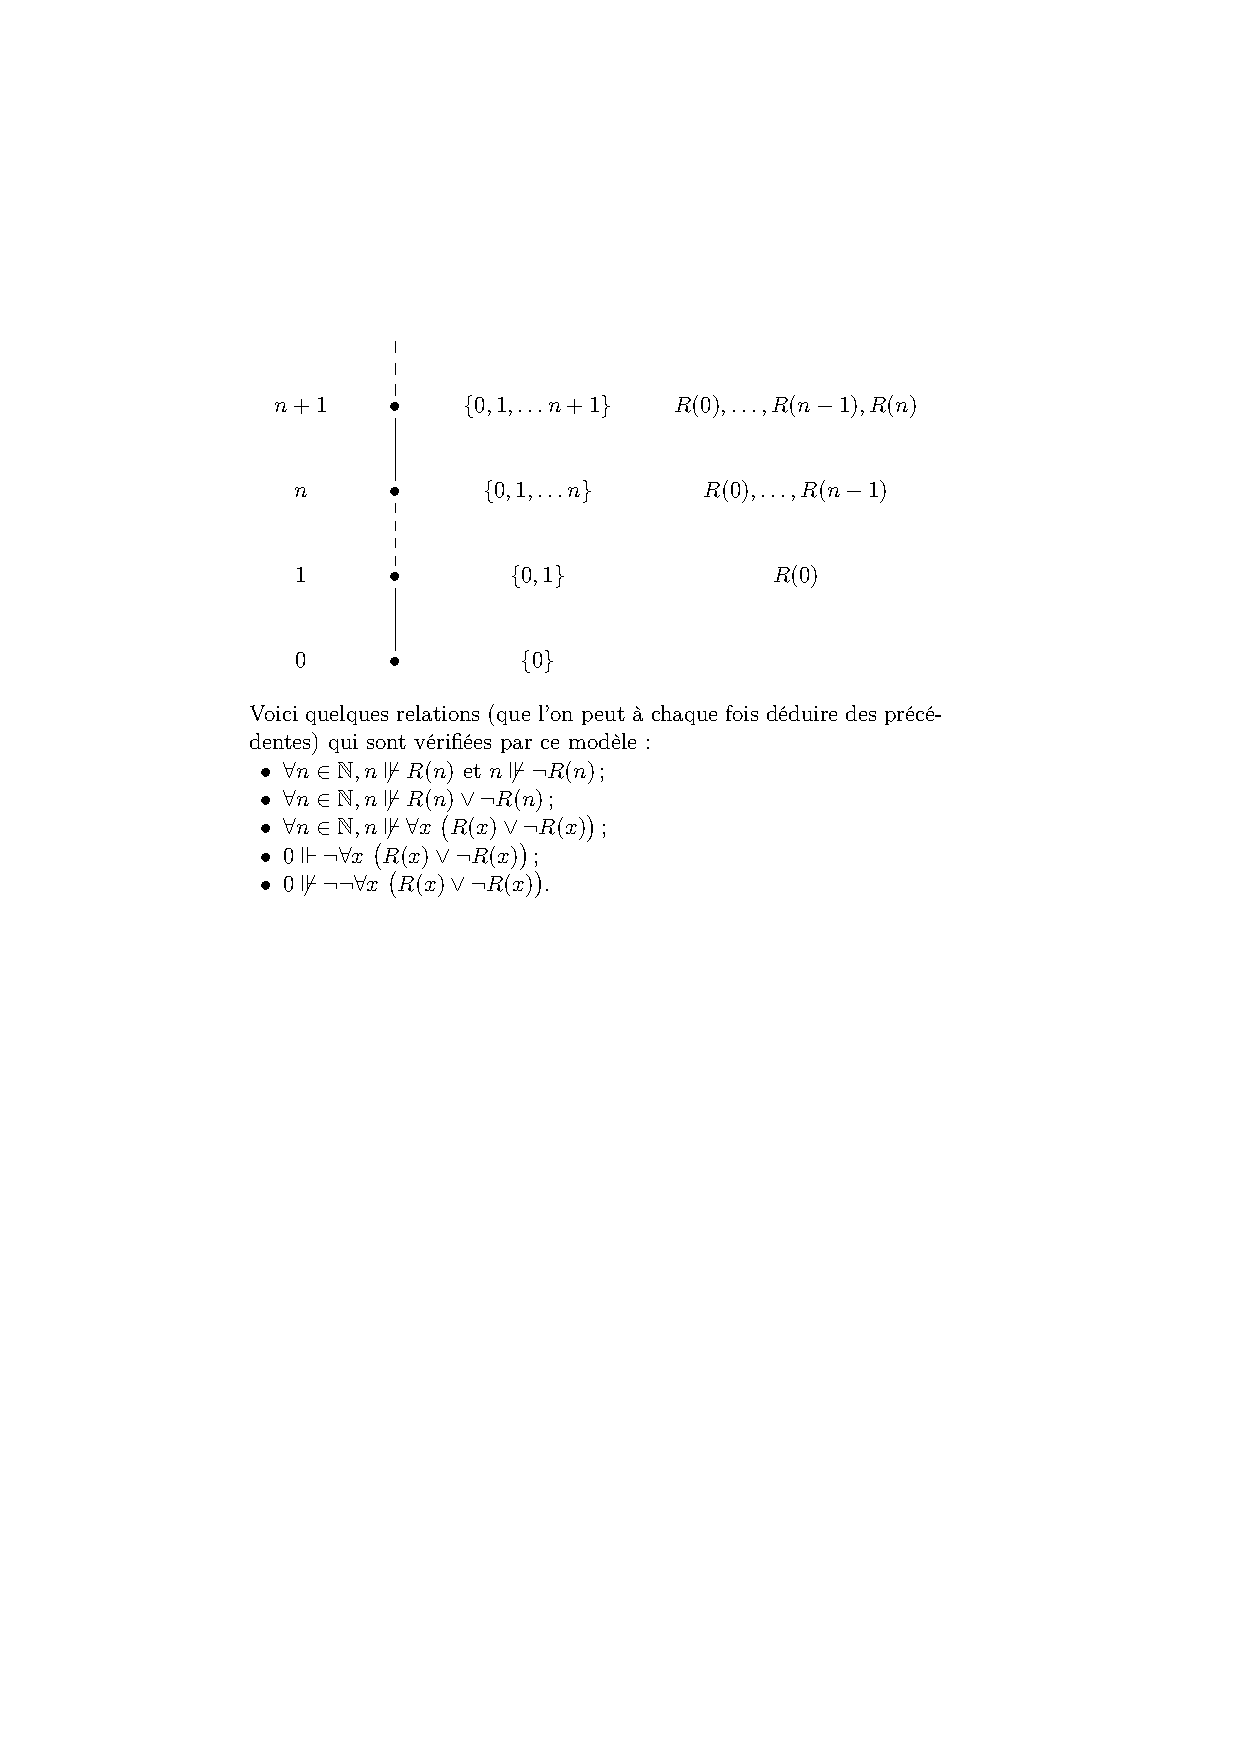
\includegraphics[width=0.32\textwidth]{images/kripke.pdf}
\end{figure}

\begin{figure}[H]
    \centering
    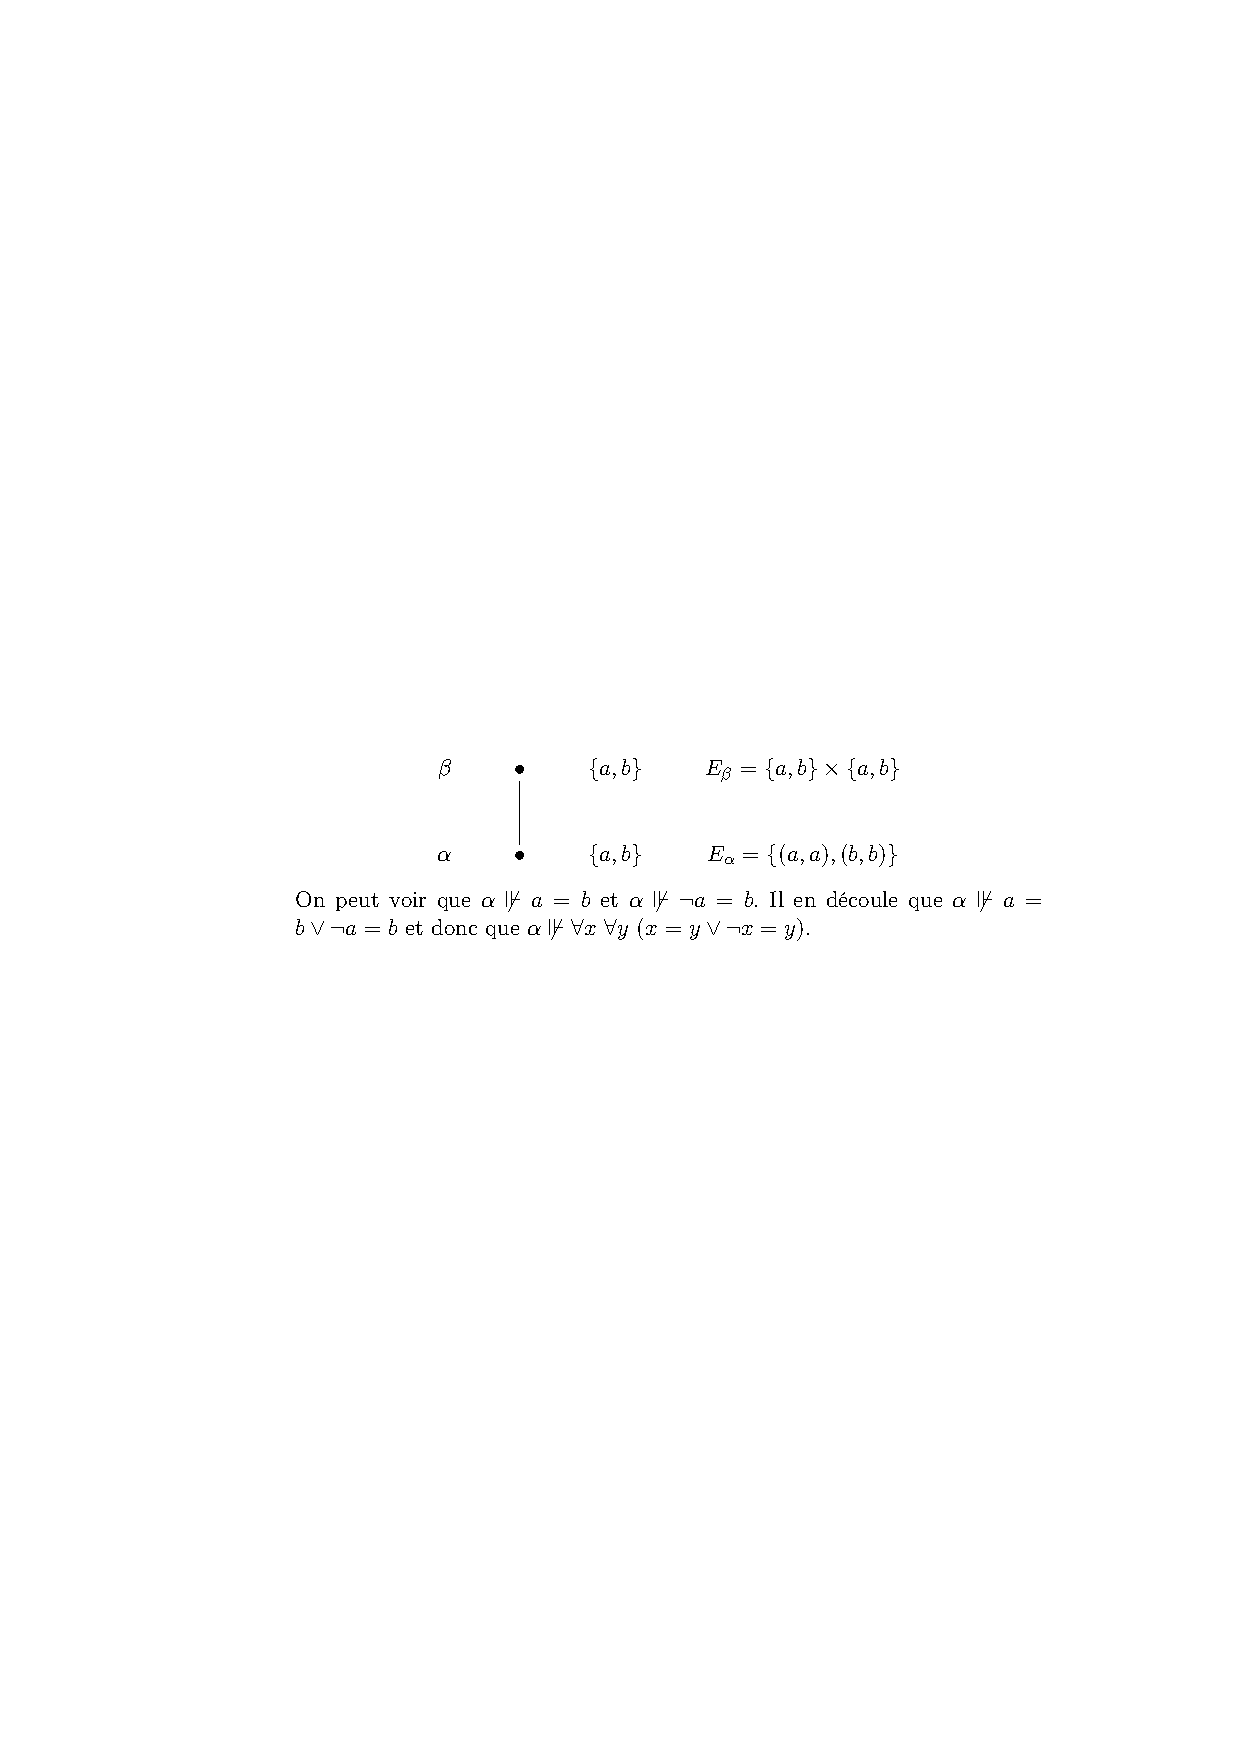
\includegraphics[width=0.32\textwidth]{images/kripke2.pdf}
\end{figure}

\section{Théorème de complétude}

\begin{thm}{12.1}[Complétude de la logique minimale] Soit $\Gamma$ une théorie et $\phi$ une formule. Alors $\Gamma \models_m \phi \iff \Gamma \vdash_m \phi$.\end{thm}

\begin{defn}{12.4}[Non-contradiction]  Un théorie $\Gamma$ est dite non-contradictoire ssi $\Gamma \not\vdash_c \bot$.\end{defn}

\begin{thm}{12.6}[Complétude bis] Une théorie est non-contradictoire ssi elle est consistante.\end{thm}

\end{multicols}
\end{document}
